\section{The DOREMUS Resource In Use} \label{sec:use}
We proceed to discuss aspects related to the use of the resources, starting with their exploration and search.

{\texttt{Overture}: {\it an Exploratory Search Engine.}} We develop \textsc{Overture} (Ontology-driVen Exploration and Recommendation of mUsical REcords), a prototype of an exploratory search engine for DOREMUS data, available at \url{http://overture.doremus.org}. The application makes requests directly to the SPARQL endpoint and provides information in a web user interface (UI).

\begin{figure}[t]
 \centerline{
 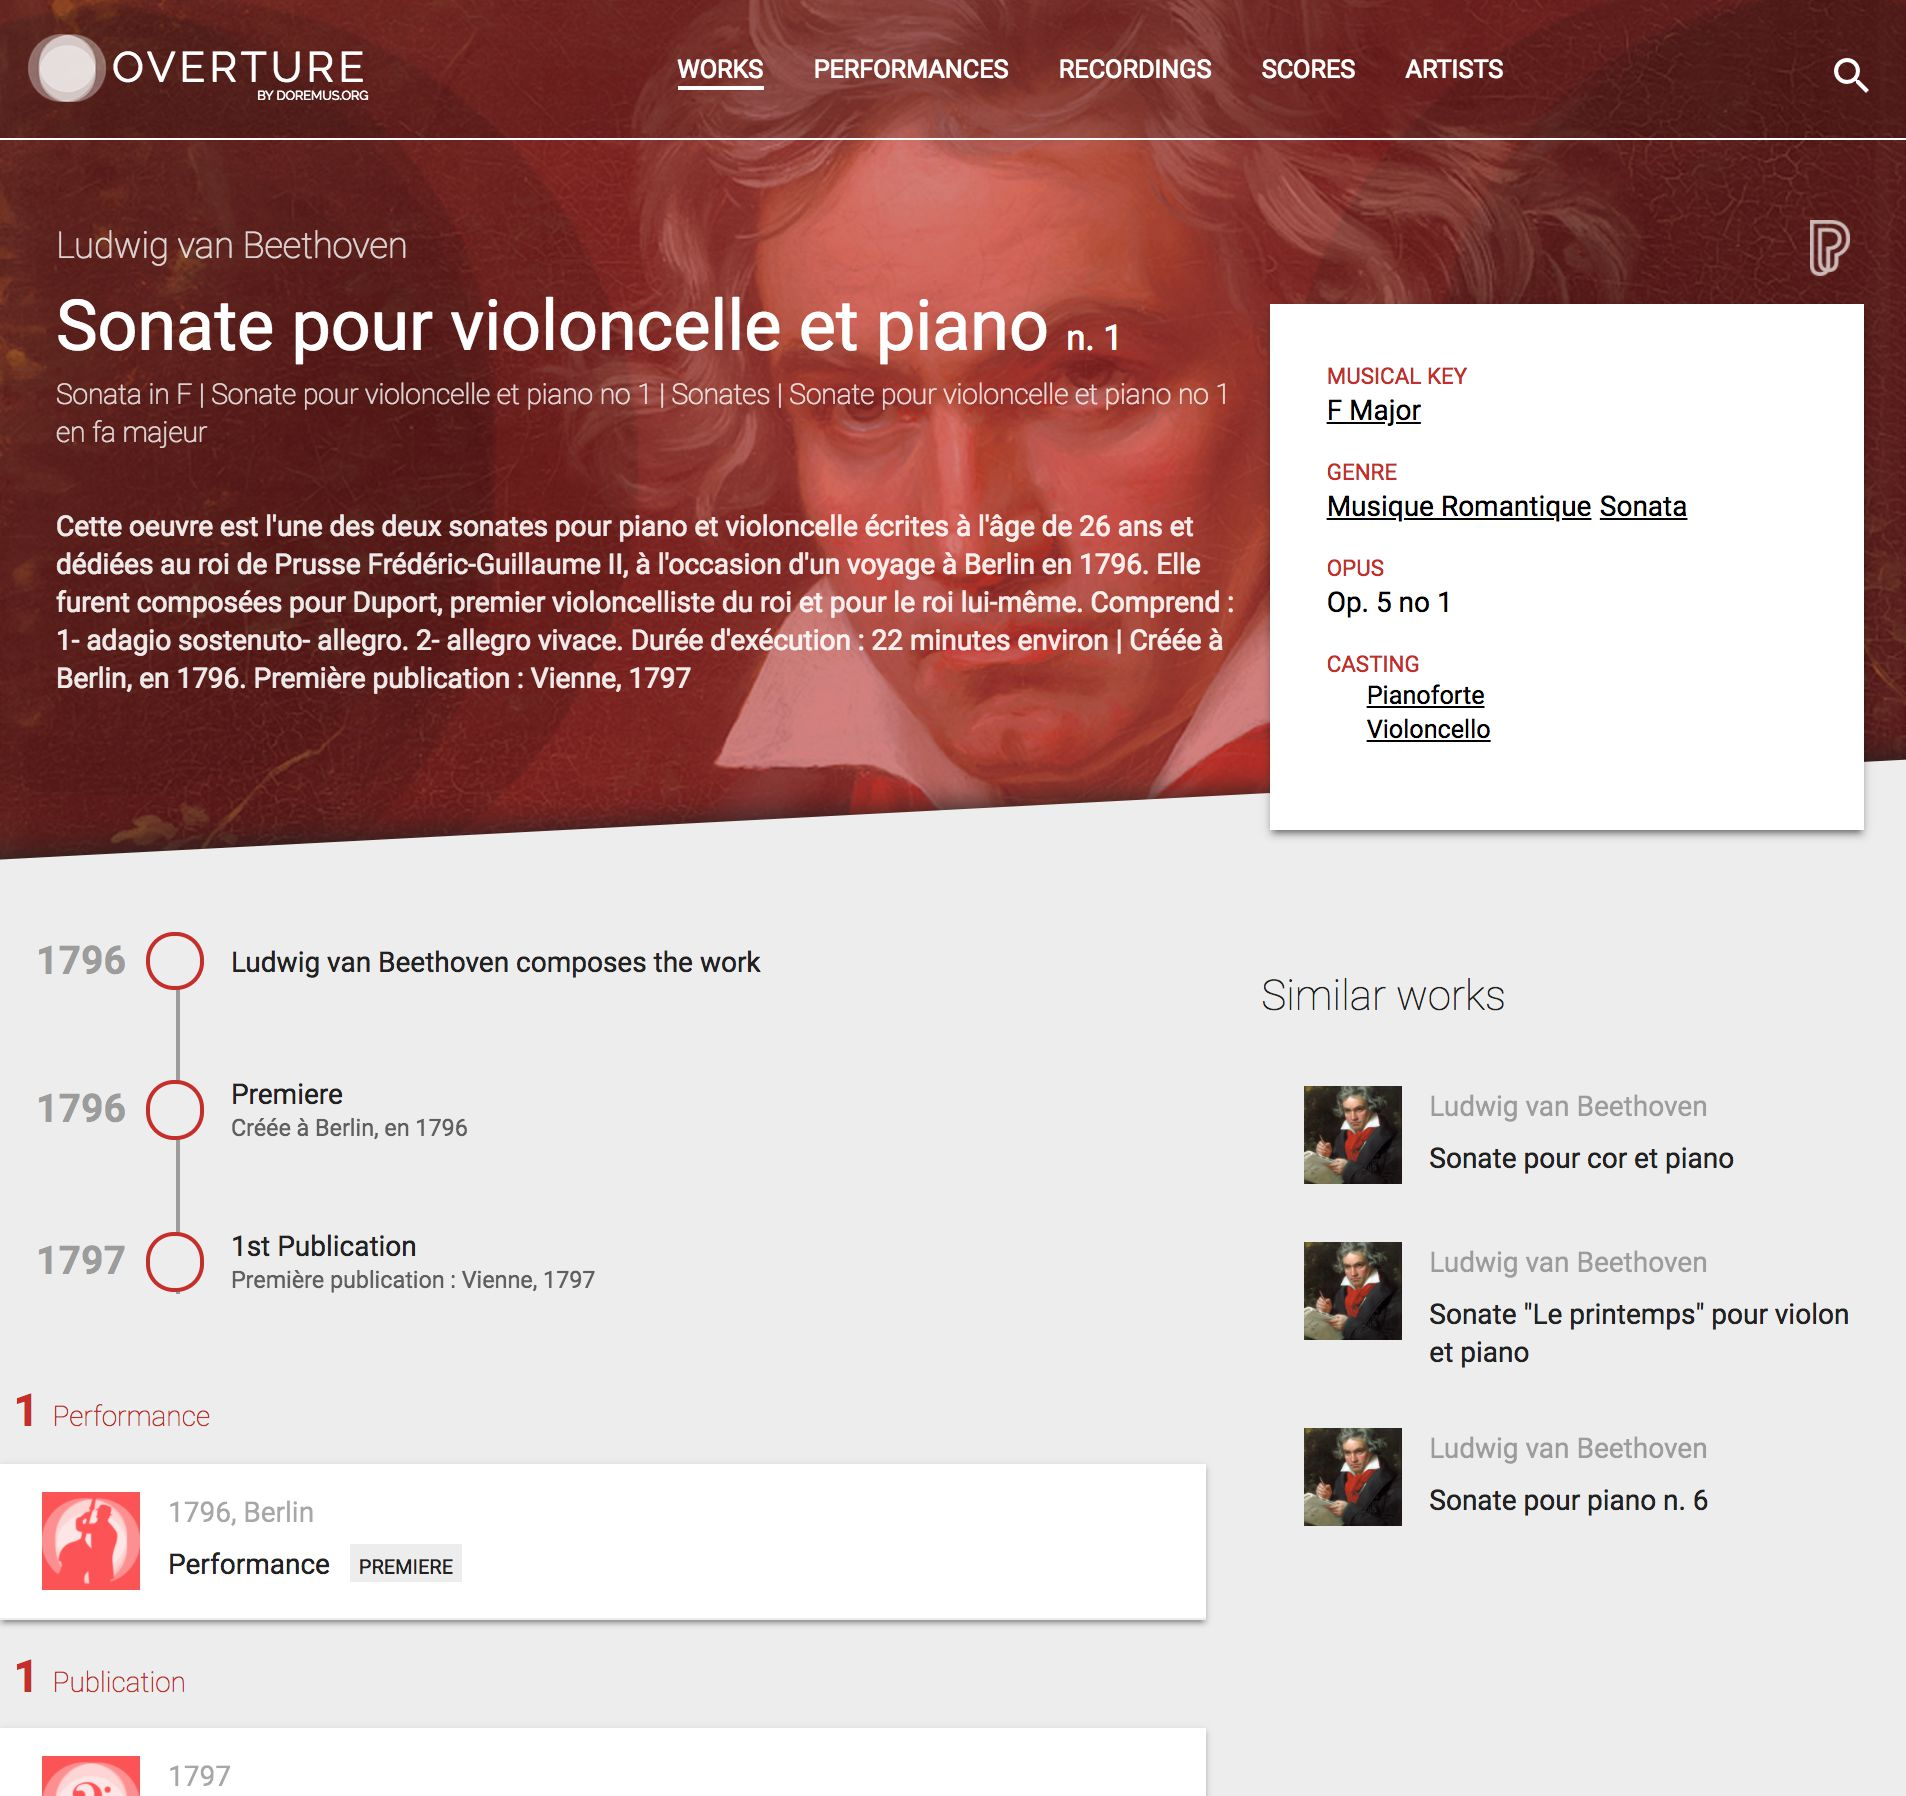
\includegraphics[width=10cm]{img/overture-sonata.jpg}}
 \caption{The detail of an expression in \textsc{Overture}}
 \label{fig:overture-detail}
\end{figure}

At the top of the UI, the menu bar allows the user to navigate between the main concepts of the DOREMUS model: expression, performance, score, recording, artist. Fig.~\ref{fig:overture-detail} represents Beethoven's \textit{Sonata for piano and cello n.1} as seen in \textsc{Overture}. Aside from the different versions of the title, the composer and a textual description, the page provides details on the information we have about the work, like the musical key, the genres, the intended MoP, the opus number. When these values come from a controlled vocabulary, a link is present in order to search for expressions that share the same value, for example, the same genre or the same musical key. A timeline shows the most important events in the story of the work (the composition, the premiere, the first publication). Other performances and publications can be represented below. 

The richness of the DOREMUS model offers to the end-user the chance to perform a detailed advanced search. All expressions (works) are searchable by facets, that include the title and the composer, but also keys, genres, detailed castings, making it possible to select very precise subsets of data, like all sonatas (genre) that involve a clarinet and a piano (MoPs). The hierarchical properties in the controlled vocabulary allow the smart retrieval not only of the entity that match exactly the chosen value (i.e. \textit{Strings}), but also any of its narrower concepts (i.e. \textit{violin}, \textit{cello}, etc.).

A {work-in-progress} recommendation system is also implemented in \texttt{Overture} in order to suggest to the final user different works to discover. The recommended works have similar properties to the current one, like the genre, the composer and the foreseen instruments. The recommendation is realized by computing knowledge graph embeddings using \textit{node2vec}~\cite{node2vec-kdd2016} on the DOREMUS knowledge graph and selecting the closer works using the euclidean distance~\cite{lisena2017artistsimilarity}.

Other client applications that also make use of the DOREMUS dataset include CityMus~\cite{lisena:iswc2017}, a mobile application that generates Spotify playlist composed of DOREMUS tracks based on the surrounding important buildings of a geo-localized user in a city. More precisely, interesting paths in the DBpedia knowledge base between POIs and composer are sought and shown to the end user in order to explain the recommendation. We also develop a chatbot that is capable of answering trivia questions in classical music.\footnote{\url{https://chatbot.doremus.org}}

\textit{Current Users and Impact.} The DOREMUS resource is currently used by librarians internally within each partner institution and across the three institutions, allowing for the fast retrieval of results for complex queries (see Table \ref{tab:links} for a link to examples). Thanks to the exploratory search engine, the DOREMUS data is open for access to a  wide community of musicians, music theorists, connoisseurs and amateurs, who do not need to have any technical expertise in order to query the RDF graphs. The controlled vocabularies and the DOREMUS ontology are also being endorsed by IFLA, as a de-facto standard for this community. The French National Library, per its conservation mission, guarantees that the DOREMUS resources will always be accessible and maintained.

Our goal is also to use the resources for both pedagogical and editorial purposes. The recommendation system that is currently under development will assist the creation of playlists for radios, allowing to group works together by very specific criteria, or to uncover rare works and provide insights about possible relations between composers, genres, events, etc.

We contribute to the semantic web community at large by providing open source implementations of novel and generic tools for data linking and fusion. We foster the adoption of semantic web technologies via the publication of numerous pedagogical materials, aiming to guide and encourage other cultural institutions to reuse the DOREMUS model and vocabularies and reproduce our data production framework (see Table \ref{tab:links}), as similar initiatives exist in other fields \cite{villazon2011methodological}.